\textbf{Newton Polygons} \\
$v(a)=-\log\pabs{a}$ for $a\in\Q_p^*$.
Newton polygon of $a_0+a_1x+\dotsb+a_nx^n$ is lower convex hull of $\brace{(i,v(a_i))}$.

\thm Let $f(x)=a_0+\dotsb+a_nx^n\in\Q_p[x]$ be a polynomial of degree $n$.
Say $(r,v(a_r))$ and $(s,v(a_s))$ are the endpoints of a line segment in the Newton polygon of $f(x)$, of slope $-m$.
Then $f(x)$ has (in some extension of $\Q_p$) $\abs{r-s}$ roots $\alpha_i$ with $\pabs{a_i}=p^{-m}$.

\note The Galois group of $f(x)$ does not change the valuation of roots of $f(x)$.
Thus, this theorem tells us that line segments in the Newton polygon correspond to factors of $f(x)$ in $\Q_p[x]$. \\
\pf Assume without loss of generality that $a_n=1$. \\
Order the roots of $f(x)$ as follows:
\begin{gather*}
\begin{array}{r@{\,}l@{\,}r}
	\alpha_1,\dotsc,\alpha_{t_1} & \leftarrow v(\alpha_i) = m_1 & \multirow{2}{*}{$>m_1$} \\
	\alpha_{t_1+1},\dotsc,\alpha_{t_2} & \leftarrow v(\alpha_i) = m_2 \\
	\vdots\qquad \\
	\alpha_{t_r+1},\dotsc,\alpha_n & \leftarrow v(\alpha_i) = m_{r+1} & > m_r
\end{array} \\
\begin{aligned}
	\text{so } v(a_n) &= 0 \\
	v(a_{n-1}) &\geq \min\brace{v(\alpha_i)} = m_1 \\
	v(a_{n-1}) &\geq \min\brace{v(\alpha_i\alpha_j)} = 2m_1 \\
	&\eqvdots \\
	v(a_{n-t_1}) &= t_1m_1 \\
	v(a_{n-t_1-1}) &\geq t_1m_1+m_2 \\
	&\eqvdots \\
	v(a_{n-t_1-t_2}) &= t_1m_1 + (t_2-t_1)m_2
\end{aligned}
\end{gather*}
Continuing in this fashion, one sees that the Newton polygon of $f(x)$ has vertices
\[ (n-t_0,t_1m_1+(t_2-t_1)m_2+\dotsb+(t_c-t_{c-1})m_c), \]
and has $r+1$ segments of slopes $-m_1$, $-m_2$, $\dotsc$, $-m_{r+1}$. \qed

\eg $x^2+x-6$, $\Q_3$.
\[ 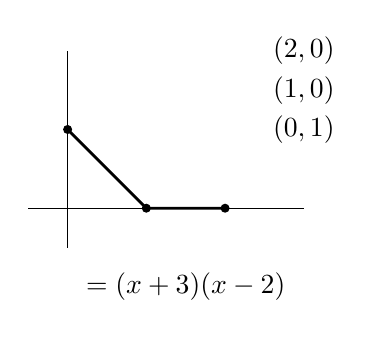
\begin{tikzpicture}[dot/.style={draw,fill,circle,inner sep=1pt}]
	\draw[-] (-0.5,0) -- (3,0);
	\draw[-] (0,-0.5) -- (0,2);
	\node[dot] at (0,1) {};
	\node[dot] at (1,0) {};
	\node[dot] at (2,0) {};
	\draw[line width=1pt] (0,1) -- (1,0) -- (2,0);
	\node at (1.5,-1) {$=(x+3)(x-2)$};
	\node at (3,2) {$(2,0)$};
	\node at (3,1.5) {$(1,0)$};
	\node at (3,1) {$(0,1)$};
\end{tikzpicture} \]
\thm Assume that the Newton polygon of $f(x)$ intersects $\Z^2$ in exactly two points.
Then $f(x)$ is irreducible in $\Q_p[x]$. \\
\pf Say $f(x)=g(x)h(x)$, and assume without loss of generality that $f$, $g$, $h$ are all monic.
We know that the Newton polygon of $f(x)$ is a single line segment of slope $m$, since the Newton polygon only has vertices at lattice points.
Say $\deg(f)=n$.

So $v(\alpha)=m$ for all roots $\alpha$ of $f$, and thus for all roots of $g$ and $h$, too.  If $\deg(g)=d$, then $\pabs{g(0)}=p^{-dm}$ and $\pabs{h(0)}=p^{-(n-d)m}$.
The Newton polygon joins $(n,0)$ to $(0,nm)$, which contains the point $(d,(n-d)m)$.
Thus, either $d=n$ or $d=0$, and so $f(x)$ is irreducible. \qed

So $x^5+2x^4+4$ is irreducible over $\Q_2$, because its Newton polygon has exactly 2 lattice points, one at each end.
